% Auto-generated by make_supplementary_figure.py — re-run after picking more examples.
% Requires \usepackage{graphicx} and \usepackage{caption} in the preamble.
\begin{figure*}[t]
\centering
\begin{tabular}{ccc}
\textbf{Reference} & \textbf{Rotated (pre-denoise)} & \textbf{Denoised (ours)} \\[4pt]
  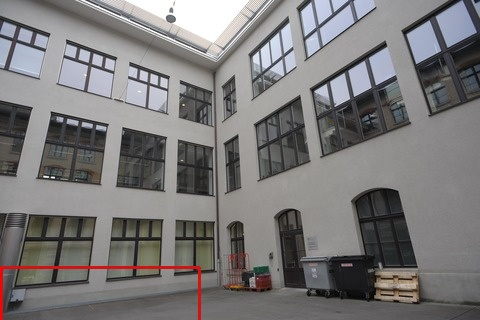
\includegraphics[width=0.30\linewidth]{supplementary_figures/difix3d_pics/eth3d_courtyard_345_0_ref.jpg} &
  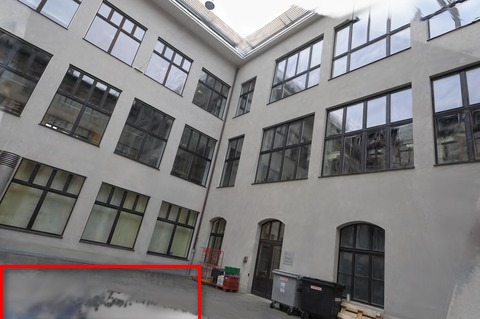
\includegraphics[width=0.30\linewidth]{supplementary_figures/difix3d_pics/eth3d_courtyard_345_0_raw.jpg} &
  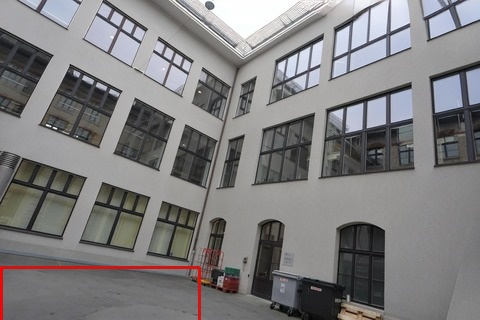
\includegraphics[width=0.30\linewidth]{supplementary_figures/difix3d_pics/eth3d_courtyard_345_0_denoised.jpg} \\
  \multicolumn{3}{c}{\scriptsize eth3d / courtyard / 345°, score 4.25} \\[4pt]
  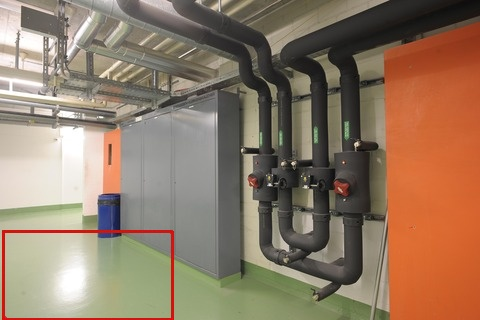
\includegraphics[width=0.30\linewidth]{supplementary_figures/difix3d_pics/eth3d_pipes_345_1_ref.jpg} &
  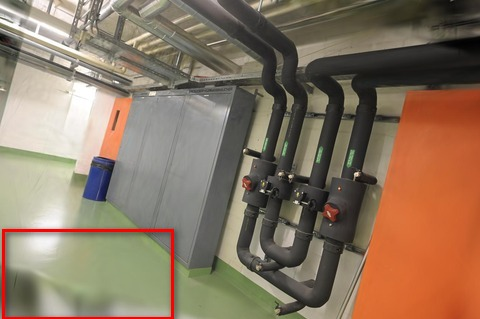
\includegraphics[width=0.30\linewidth]{supplementary_figures/difix3d_pics/eth3d_pipes_345_1_raw.jpg} &
  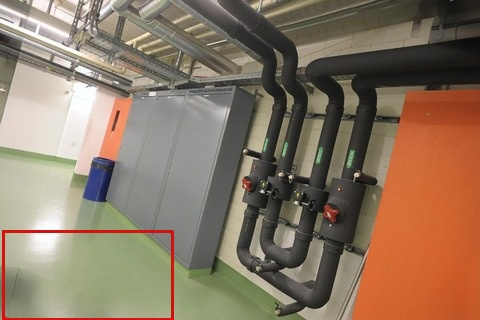
\includegraphics[width=0.30\linewidth]{supplementary_figures/difix3d_pics/eth3d_pipes_345_1_denoised.jpg} \\
  \multicolumn{3}{c}{\scriptsize eth3d / pipes / 345°, score 4.25} \\[4pt]
  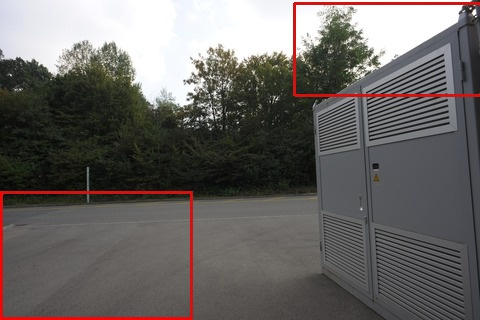
\includegraphics[width=0.30\linewidth]{supplementary_figures/difix3d_pics/eth3d_electro_330_2_ref.jpg} &
  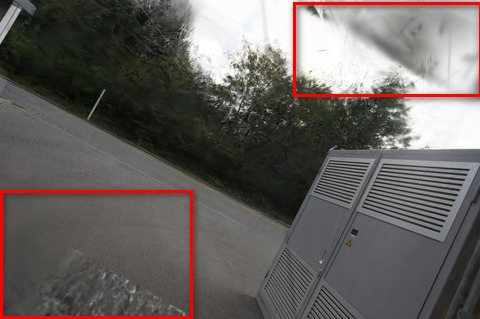
\includegraphics[width=0.30\linewidth]{supplementary_figures/difix3d_pics/eth3d_electro_330_2_raw.jpg} &
  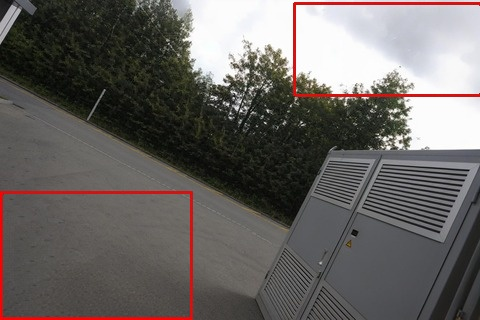
\includegraphics[width=0.30\linewidth]{supplementary_figures/difix3d_pics/eth3d_electro_330_2_denoised.jpg} \\
  \multicolumn{3}{c}{\scriptsize eth3d / electro / 330°, score 4.20} \\[4pt]
  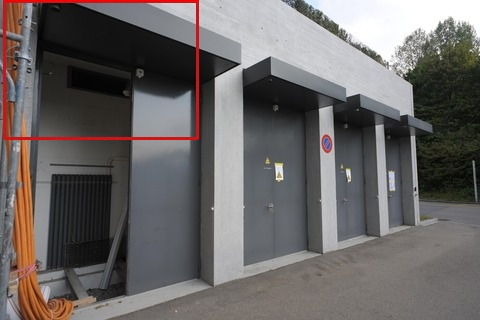
\includegraphics[width=0.30\linewidth]{supplementary_figures/difix3d_pics/eth3d_electro_60_3_ref.jpg} &
  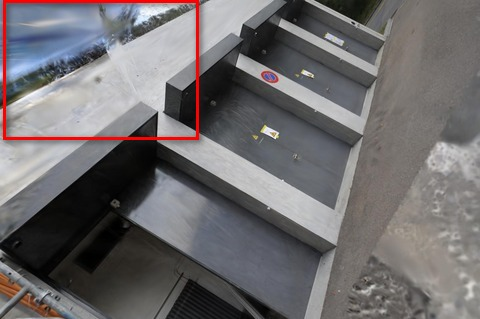
\includegraphics[width=0.30\linewidth]{supplementary_figures/difix3d_pics/eth3d_electro_60_3_raw.jpg} &
  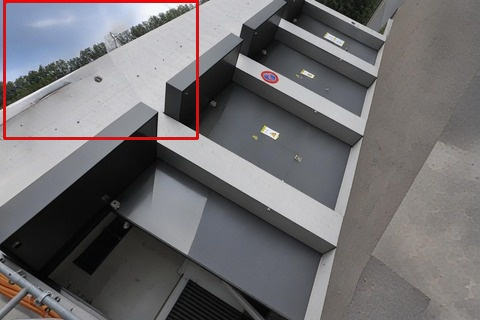
\includegraphics[width=0.30\linewidth]{supplementary_figures/difix3d_pics/eth3d_electro_60_3_denoised.jpg} \\
  \multicolumn{3}{c}{\scriptsize eth3d / electro / 60°, score 3.80} \\[4pt]
  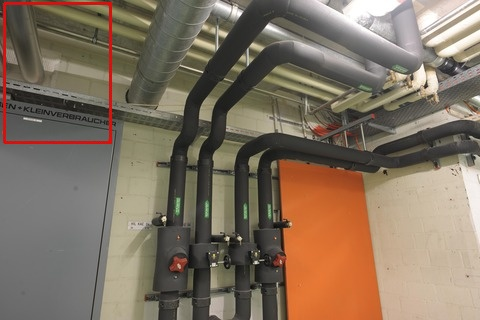
\includegraphics[width=0.30\linewidth]{supplementary_figures/difix3d_pics/eth3d_pipes_60_4_ref.jpg} &
  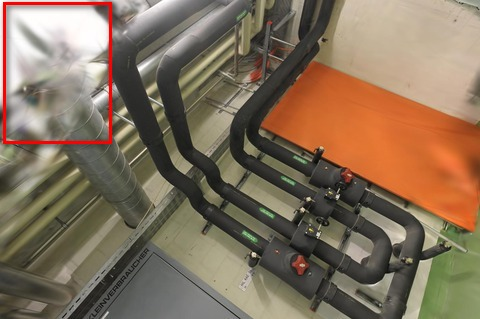
\includegraphics[width=0.30\linewidth]{supplementary_figures/difix3d_pics/eth3d_pipes_60_4_raw.jpg} &
  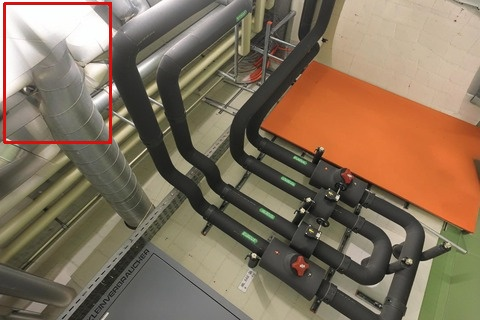
\includegraphics[width=0.30\linewidth]{supplementary_figures/difix3d_pics/eth3d_pipes_60_4_denoised.jpg} \\
  \multicolumn{3}{c}{\scriptsize eth3d / pipes / 60°, score 3.80} \\[4pt]
\end{tabular}
\caption{Qualitative examples where denoising most improved the rotated render relative to the reference view.}
\label{fig:denoise-examples}
\end{figure*}

\begin{figure*}[t]
\ContinuedFloat
\centering
\begin{tabular}{ccc}
\textbf{Reference} & \textbf{Rotated (pre-denoise)} & \textbf{Denoised (ours)} \\[4pt]
  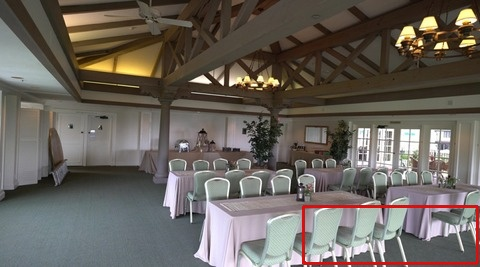
\includegraphics[width=0.30\linewidth]{supplementary_figures/difix3d_pics/tnt_Meetingroom_roll_15_5_ref.jpg} &
  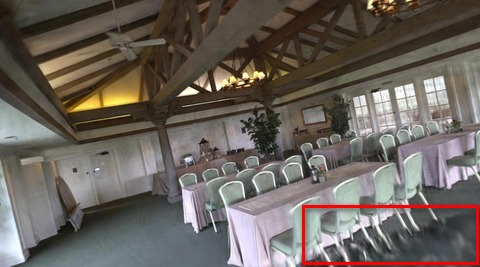
\includegraphics[width=0.30\linewidth]{supplementary_figures/difix3d_pics/tnt_Meetingroom_roll_15_5_raw.jpg} &
  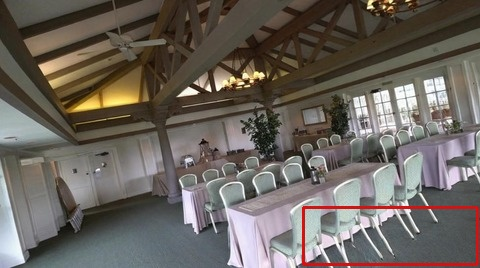
\includegraphics[width=0.30\linewidth]{supplementary_figures/difix3d_pics/tnt_Meetingroom_roll_15_5_denoised.jpg} \\
  \multicolumn{3}{c}{\scriptsize tnt / Meetingroom / roll 15°, score 4.20} \\[4pt]
  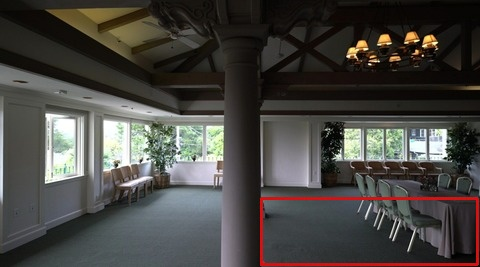
\includegraphics[width=0.30\linewidth]{supplementary_figures/difix3d_pics/tnt_Meetingroom_roll_15_6_ref.jpg} &
  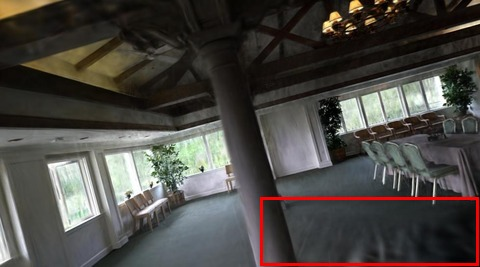
\includegraphics[width=0.30\linewidth]{supplementary_figures/difix3d_pics/tnt_Meetingroom_roll_15_6_raw.jpg} &
  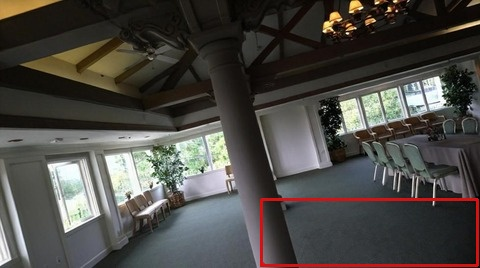
\includegraphics[width=0.30\linewidth]{supplementary_figures/difix3d_pics/tnt_Meetingroom_roll_15_6_denoised.jpg} \\
  \multicolumn{3}{c}{\scriptsize tnt / Meetingroom / roll 15°, score 4.20} \\[4pt]
  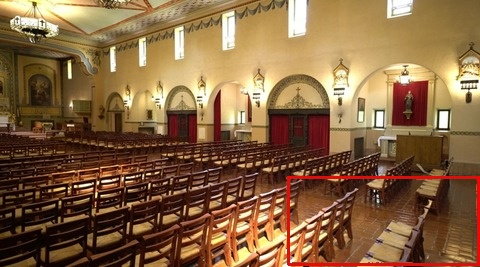
\includegraphics[width=0.30\linewidth]{supplementary_figures/difix3d_pics/tnt_Church_roll_15_7_ref.jpg} &
  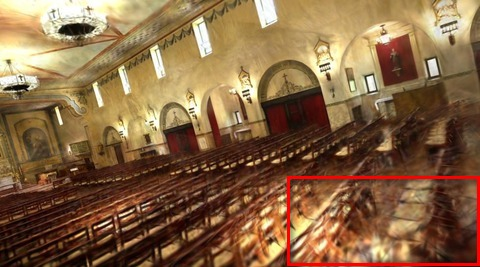
\includegraphics[width=0.30\linewidth]{supplementary_figures/difix3d_pics/tnt_Church_roll_15_7_raw.jpg} &
  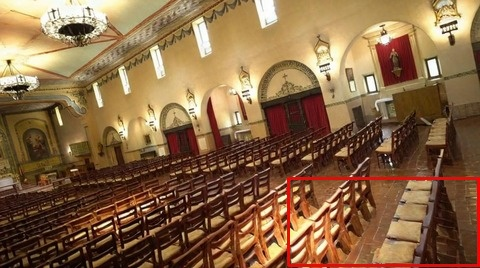
\includegraphics[width=0.30\linewidth]{supplementary_figures/difix3d_pics/tnt_Church_roll_15_7_denoised.jpg} \\
  \multicolumn{3}{c}{\scriptsize tnt / Church / roll 15°, score 4.00} \\[4pt]
  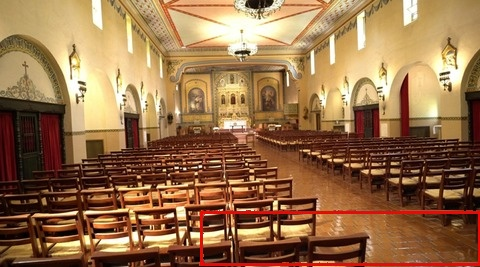
\includegraphics[width=0.30\linewidth]{supplementary_figures/difix3d_pics/tnt_Church_roll_15_8_ref.jpg} &
  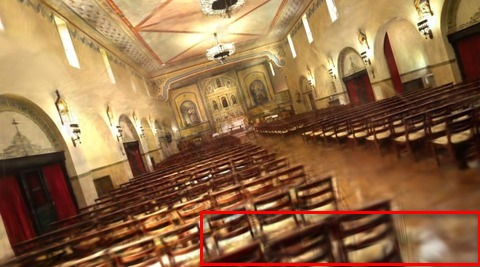
\includegraphics[width=0.30\linewidth]{supplementary_figures/difix3d_pics/tnt_Church_roll_15_8_raw.jpg} &
  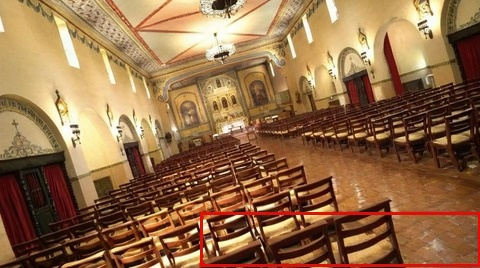
\includegraphics[width=0.30\linewidth]{supplementary_figures/difix3d_pics/tnt_Church_roll_15_8_denoised.jpg} \\
  \multicolumn{3}{c}{\scriptsize tnt / Church / roll 15°, score 4.00} \\[4pt]
\end{tabular}
\caption{(continued)}
\end{figure*}

\begin{figure*}[t]
\centering
\begin{tabular}{cc}
    \textbf{VGGT} & \textbf{Ours} \\[4pt]
    
    % --- Pair 1: Chess ---
    \includegraphics[width=0.39\linewidth]{Figures/pointcloud_images/publication_figure_chess_bad.png} &
    \includegraphics[width=0.35\linewidth]{Figures/pointcloud_images/publication_figure_chess_good.png} \\
    \multicolumn{2}{c}{\scriptsize Chess} \\[4pt]

    % --- Pair 2: Church ---
    \includegraphics[width=0.36\linewidth]{Figures/pointcloud_images/publication_figure_church_bad.png} &
    \includegraphics[width=0.35\linewidth]{Figures/pointcloud_images/publication_figure_church_good.png} \\
    \multicolumn{2}{c}{\scriptsize Church} \\[4pt]

    % --- Pair 3: Pumpkin ---
    \includegraphics[width=0.41\linewidth]{Figures/pointcloud_images/publication_figure_pumpkin_bad.png} &
    \includegraphics[width=0.35\linewidth]{Figures/pointcloud_images/publication_figure_pumpkin_good.png} \\
    \multicolumn{2}{c}{\scriptsize Office} \\[4pt]

    % --- Pair 4: Truck ---
    \includegraphics[width=0.35\linewidth]{Figures/pointcloud_images/publication_figure_truck_bad.png} &
    \includegraphics[width=0.35\linewidth]{Figures/pointcloud_images/publication_figure_truck_good.png} \\
    \multicolumn{2}{c}{\scriptsize Truck} \\[4pt]
\end{tabular}
\caption{Qualitative comparison of point cloud reconstructions across different scenes.}
\label{fig:pointcloud_comparison}
\end{figure*}